\documentclass[12pt]{article}

\usepackage{sbc-template}

\usepackage{graphicx,url}

%\usepackage[brazil]{babel}   
\usepackage[latin1]{inputenc}  
\usepackage{amsthm}
\usepackage{amssymb}
\usepackage{amsmath}
\usepackage{amsfonts}
\usepackage{alltt}


\newcommand{\Pow}{\, \widehat{} \,\,}
\newcommand{\Match}[3]{\mathrm{match} \;\, #1\;#2\;#3}
\newcommand{\Matchf}[4]{\mathrm{match} \;\, #1\;#2\;#3\;#4}
\newcommand{\Matchl}[4]{\mathrm{match}_L \;\, #1\;#2\;#3\;#4}
\newcommand{\Matchlk}[5]{\mathrm{match}_L \;\, #1\;#2\;#3\;#4\;#5}
\newcommand{\Matchrec}[5]{\mathrm{match} \;\, #1\;#2\;#3\;#4\;#5}
\newcommand{\Nothing}{{\tt fail}}
\newcommand{\Just}[1]{\mbox{#1}}
\newcommand{\Justc}[2]{(\mbox{#1},\,#2)}
\newcommand{\Striple}[3]{(#1,\,#2,\,#3)}
\newcommand{\Sstate}[4]{\langle#1,\,#2,\,#3,\,#4\rangle}
\newcommand{\Sstatec}[5]{\langle#1,\,#2,\,#3,\,#4,\,#5\rangle}
\newcommand{\Sfail}[1]{\mbox{\bf Fail}{\langle#1\rangle}}
\newcommand{\Sstep}[4]{#1 & \xrightarrow{#2} & #3 & #4\\}
\newcommand{\Sstepp}[4]{#1 \xrightarrow{#2} #3\\}
\newcommand{\Ia}[2]{\mbox{{\scriptsize {\tt #1} $#2$}}}
\newcommand{\Iaa}[3]{\mbox{{\scriptsize {\tt #1} $#2$ $#3$}}}
\newcommand{\Fail}{\mbox{\bf Fail}}
\newcommand{\Hd}[1]{\mbox{hd}(#1)}
\newcommand{\Sub}{{s}}
\newcommand{\Subb}{{s_1}}
\newcommand{\Subi}{\Sub [i]}
\newcommand{\Subbi}{\Subb [i]}
\newcommand{\MathN}[1]{\mbox{\emph{#1}}}
\newcommand{\Nat}{\mbox{\bf N}}
\newcommand{\myarrow}{\xrightarrow{\;\;\;\;\;}}
\newcommand{\myarrowstar}{\xrightarrow{\;\;*\;\;}}
\newcommand{\fivespaces}{\;\;\;\;\;}
\newcommand{\tenspaces}{\fivespaces\fivespaces}
\newcommand{\twentyspaces}{\tenspaces\tenspaces}
\newcommand{\thirtyspaces}{\twentyspaces\tenspaces}
\newcommand{\fortyspaces}{\twentyspaces\twentyspaces}
\newcommand{\interf}{\fivespaces}
\newcommand{\mylabel}[1]{\ \textbf{(#1)}}
\newcommand{\chmath}[1]{\mbox{`}#1\mbox{'}}

\newcommand{\Eval}[1]{\mathrm{eval} \; #1}
\newcommand{\Esimple}[2]{\mathrm{esimp} \; #1\;#2}
\newcommand{\Efunction}[2]{\mathrm{efunc} \; #1\;#2}
\newcommand{\Efold}[2]{\mathrm{efold} \; #1\;#2}
\newcommand{\Cconst}[1]{\mathrm{Cconst} \; #1}
\newcommand{\Csimple}[2]{\mathrm{Csimple} \; (#1,\,#2)}
\newcommand{\Cfunc}[1]{\mathrm{Cfunc} \; #1}
\newcommand{\Cfold}[1]{\mathrm{Cfold} \; #1}
\newcommand{\Cclose}[1]{\mathrm{Cclose} \; #1}
\newcommand{\Emptyl}{\{\}}
\newcommand{\Mapl}{map_{s \rightarrow l}}
\newcommand{\Pcap}[2]{\langle#1,\,#2\rangle}
\newcommand{\Pcapp}[3]{\langle#1,\,#2,\,#3\rangle}
\newcommand{\Concatl}{\,}

\newtheorem{proposition}{Proposition}

\sloppy

\title{Efficient List Matching using PEGs}

\author{S�rgio Medeiros\inst{1}, Fabio Mascarenhas\inst{1}, Roberto Ierusalimschy\inst{1} }


\address{Department of Computer Science -- PUC-Rio -- Rio de Janeiro -- Brazil
  \email{\{smedeiros,roberto\}@inf.puc-rio.br, mascarenhas@acm.org}
}

\begin{document} 

\maketitle

\begin{abstract}
Parsing Expression Grammars (PEGs) are a recognition-based foundation
for describing syntax that renewed interest in top-down parsing
approaches. We extend the definition of PEGs to support the matching
of structured data in the form of lists, with a corresponding operational semantics.
We also extend a virtual parsing machine from a previous work where
each PEG can be transformed to a program for this machine, and extend the
previous correctness proofs of this transformation for the new list patterns, along
with possible optimizations. We also present an approach for formally adding 
semantic actions to PEGs and their parsing machine programs. Benchmarks validate
the effectiveness of our optimizations and the efficiency of our approach compared
to other PEG-based tool.
\end{abstract}

%\keywords{parsing machine, Parsing Expression Grammars, pattern matching, virtual machines}

\section{Introduction}

Parsing Expression Grammars (PEGs)~\cite{ford:peg} are a formalism for
language recognition which renewed interest in top-down parsing
approaches. The PEG formalism gives a convenient syntax for describing
top-down parsers for unambiguous languages. The core of the formalism
is a form of limited backtracking via \emph{ordered choice}. The
limited backtracking gives PEGs the property of composability, meaning
that a PEG can be used by another PEG just by making sure the names of
their productions do not clash. This also lets PEG implementations
integrate cleanly with hand-written parsers. These properties make
PEGs very attractive for building dynamically-extensible parsers.

LPEG~\cite{roberto:lpeg} is a pattern-matching tool for the Lua
language ~\cite{pil2} that uses PEGs to describe patterns instead of
the more popular Perl-like ``regular expressions" (regexes).  The
implementation of LPEG uses a \emph{virtual parsing machine}, where
each pattern translates to a program for this
machine~\cite{dls:lpeg}. LPEG builds these programs at runtime,
dynamically composing smaller programs into bigger programs, thus
taking advantage of the composability of PEGs. PEGs limited
backtracking is also reflected on this parsing machine through its use
of a stack to manage backtrack information.

This paper is a continuation of a previous work~\cite{dls:lpeg} where
we presented an alternative operational semantic for PEGs (based on
natural semantics), and a formal specification of the parsing machine,
along with a correctness proof for our transformation of PEGs to
programs of the machine.

Both the original PEG formalism and our previous parsing machine
assume that the subject a PEG recognizes is a string of characters. In
this paper, we extend both formalisms to parse structured data in the
form of Lisp-style lists (a possibly empty list where each element can
be an atom or another list). We show that our previous results hold
when matching lists or slices of lists that are isomorphic to strings,
and give proofs for the correctness of the translation of our new
constructions.

Extending PEGs to match structured data make PEGs useful for a larger
part of the compilation pipeline. A PEG-based
scannerless parser can construct an abstract syntax tree, and
PEG-based tree walkers and transformers can implement analysis and
optimization passes on this tree, then either compiling it to
a target language (either an intermediate language close to machine
code or a naive translation to machine code).
Using the same abstraction (PEGs) for the
whole pipeline of simple domain-specific languages can make them
easier for programmers to design and implement.

Adding a few extra instructions to the parsing machine enables
transformation of certain pattern classes to more efficient programs,
and we also present these optimizations. We restrict ourselves to
optimizations on list patterns, as our previous work has covered more
general parsing machine optimizations. For each optimization, we
present a proof of its correctness and a benchmark showing how
effective it is.

We also present an extension to the PEG formalism to include a mix of
standard pattern matchers' captures and parser generators' semantic
actions, by which we can extract useful information from structured
data, instead of just knowing if it fits a pattern.  We do this
lazily, with the match just collecting enough information to extract
captures and execute actions later (in a typical implementation, right
after the match finishes). This means that semantic actions are free
to have side-effects even in the presence of backtracking.

Finally, we review related work on parsing structured data and on
semantic actions for PEGs. We also present another set of benchmarks
comparing our extended LPEG with a PEG-based tool of similar power,
showing an order-of-magnitude improvement.

The rest of this paper is organized as follows:
Section~\ref{sec:lists} extends PEGs with list patterns;
Section~\ref{sec:machine} describes the virtual parsing machine;
proves the transformation between PEGs and their corresponding
programs for the machine is correct; Section~\ref{sec:optimizations}
describes optimizations for list patterns in our machine;
Section~\ref{sec:captures} extends PEGs with lazy semantic actions and
shows how to execute them; Section~\ref{sec:related} reviews some
related work; finally, Section~\ref{sec:conclusions} summarizes our
results.

\section{Extending PEGs for Lists}
\label{sec:lists}

In~\cite{dls:lpeg}, we described a \texttt{match} relation for PEGs,
where we defined the relation \texttt{match} on $\mathrm{Grammar}
\times \mathrm{Pattern} \times \Sigma^{*} \times \mathcal{N} \times
(\mathcal{N} \cup \{\Nothing\})$.  Given a grammar (a map from
variables to patterns), a pattern, a subject string, and a position
(the subject starts at position $1$), the relation gives us either the
position after the match (possibly the length of the subject plus $1$)
or \Nothing, depending on whether the pattern matches the subject or
not. We use $\Matchf{G}{p}{s}{i} \leadsto j$ to indicate that $(G, p,
s, i, j) \in \texttt{match}$.

In this paper, we are considering lists to be Lisp-style lists, made
up from atoms and other lists. We will restrict ourselves to only
characters as atoms. We represent the empty list as \Emptyl. Lists are
inductively defined by the operator \emph{:} (also known as cons). If
$c$ is an atom and $l$ is a list then $c:l$ is a list, and if $l_1$
and $l_2$ are lists then $l_1:l_2$ is a list. The first argument of
$:$ is the head of the list and the second is the tail. We will use
$\{ e_1 e_2 \ldots e_n \}$ as another way to write $e_1:e_2:\ldots
:e_n:\Emptyl$.

We will use $|l|$ to represent the number of elements of list $l$, and
its inductive definition is trivial. We will use $l[i]$ to denote the
$i^{th}$ element of the list, starting from $1$, which also has a
straightforward inductive definition. List concatenation is
represented by juxtaposition ($l_1l_2$ is the list with all elements
of $l_1$ followed by all elements from $l_2$, not to be confused with
$l_1:l_2$, which is a list with $l_1$ as the first element followed by
the elements of $l_2$).

Now we can define a new relation $\texttt{match}_L$ on
$\mathrm{Grammar} \times \mathrm{Pattern} \times \mathrm{List} \times
\mathcal{N} \times (\mathcal{N} \cup \{\Nothing\})$.  This relation
gives us the position in the list after trying to match a pattern
given a starting position and a grammar, or \Nothing if the list does
not match the pattern. As with \texttt{match}, we also have a notation
$\Matchl{G}{p}{s}{i} \leadsto j$ to indicate that $(G, p, s, i, j) \in
\texttt{match}_L$.

Table~\ref{tab:patterns} presents the abstract syntax of PEG patterns
with the new \emph{list pattern} $\{p\}$, and Figure~\ref{fig:semgr}
presents an operational semantics of $\texttt{match}_L$ given as rules
on the pattern structure. Except for rules $list.1$ and $list.2$, all
semantic rules of $\texttt{match}_L$ are taken straight from
\texttt{match}. We have that $\Matchl{G}{p}{s}{i} \leadsto j$ if we
can use the rules to build a finite derivation tree for this
proposition.

%
\begin{table}
\centering
\begin{tabular}{|c|} \hline
\chmath{.}            $\in$ Pattern  \\ %\hline
\chmath{c}            $\in$ Pattern  \\ %\hline
If $(A, p)$ $\in$ Grammar then  $A$     $\in$ Pattern  \\ %\hline
If $p$   $\in$ Pattern then      
  $p^*$, $!p$, $\&p$, and $\{p\}$  $\in$ Pattern \\ %\hline	
If $p_{1}$ and $p_{2}$ $\in$ Pattern then
 $p_{1}p_{2}$ and $p_{1}/p_{2}$ $\in$ Pattern \\ \hline
\end{tabular}
\caption{Syntax of PEG patterns}
\label{tab:patterns}
\end{table}
%

Rules $list.1$ and $list.2$ formalize the notion that a list pattern
$\{p\}$ only succeeds if the current element of the subject is also a
list and if $p$ matches this whole sublist from the first
element. Thus the pattern $\{ \chmath{a} \chmath{b} \}$ matches the
list $\{ \chmath{a} \chmath{b} \}$ but not the list $\{ \chmath{a}
\chmath{b} \chmath{c} \}$, or the atom $\chmath{a}$.

The set of character strings is isomorphic to the set of lists where
all elements are characters plus the empty list. Lets define $\Mapl$
as the natural mapping from strings to lists, that is, the empty
string maps to the empty list, and a string $\chmath{c_1} \ldots
\chmath{c_n} $ maps to $\{ \chmath{c_1} \ldots \chmath{c_n} \}$. In
other words, if $s$ is a string, $|s| = |\Mapl(s)|$ and $s[i] =
\Mapl(s)[i]$ for $1 \leq i \leq |s|$. We then have
\begin{equation*}
\Matchf{G}{p}{s}{i} \leadsto j \;\;\mbox{iff}\;\;
\Matchl{G}{p}{\Mapl(s)}{i} \leadsto j.
\end{equation*}
with a trivial inductive proof on the height of the derivation tree,
given the semantic rules are identical. In other words, our extended
semantics is identical to the regular PEG semantics when we are
dealing with string-like lists as subjects.

%%%%%%%%%%%%%%%%%%%%%%%%%%%%%%%%%%%%%%%%%%%%%%%%%%%%%%%%%%%%%%%%%%%%%%
%%%% Operational Semantics of PEG Patterns with Grammars and Lists %%%
%%%%%%%%%%%%%%%%%%%%%%%%%%%%%%%%%%%%%%%%%%%%%%%%%%%%%%%%%%%%%%%%%%%%%%

\begin{figure*}[t]
{
\footnotesize
\begin{align*}
%Matching a given character
& \textbf{Character} \tenspaces 
{\frac{s[i] = \chmath{c}}{\Matchl{g}{\chmath{c}}{s}{i} \leadsto \Just{i+1}}} \mylabel{ch.1} \tenspaces
{\frac{s[i] \neq \chmath{c}}{\Matchl{g}{\chmath{c}}{s}{i} \leadsto \Nothing}} \mylabel{ch.2} \\
%Matching any element
& \textbf{Any Element} \tenspaces
{\frac{i \leq |s|}{\Matchl{g}{.}{s}{i} \leadsto \Just{i+1}}} \mylabel{any.1} \tenspaces
{\frac{i > |s|}{\Matchl{g}{.}{s}{i} \leadsto \Nothing}} \mylabel{any.2} \\
%Not
& \textbf{Not Predicate} \tenspaces \fivespaces
{\frac{\Matchl{g}{p}{s}{i} \leadsto \Nothing} 
	{\Matchl{g}{!p}{s}{i} \leadsto \Just{i}}} \mylabel{not.1} \tenspaces
{\frac{\Matchl{g}{p}{s}{i} \leadsto \Just{i+j}}
	{\Matchl{g}{!p}{s}{i} \leadsto \Nothing}} \mylabel{not.2} \\
%And
& \textbf{And Predicate} \tenspaces \fivespaces
{\frac{\Matchl{g}{p}{s}{i} \leadsto \Just{i+j}}
	{\Matchl{g}{\&p}{s}{i} \leadsto \Just{i}}} \mylabel{and.1} \tenspaces
{\frac{\Matchl{g}{p}{s}{i} \leadsto \Nothing}
	{\Matchl{g}{\&p}{s}{i} \leadsto \Nothing}} \mylabel{and.2} \\
%Concatenation
& \textbf{Concatenation} \twentyspaces
{\frac{\Matchl{g}{p_{1}}{s}{i} \leadsto \Just{i+j} \interf \Matchl{g}{p_{2}}{s}{i+j} \leadsto \Just{i+j+k}}
{\Matchl{g}{p_{1}p_{2}}{s}{i} \leadsto \Just{i+j+k}}} \mylabel{con.1}  \\
& \fivespaces
{\frac{\Matchl{g}{p_{1}}{s}{i} \leadsto \Just{i+j} \interf \Matchl{g}{p_{2}}{s}{i+j} \leadsto \Nothing}
	{\Matchl{g}{p_{1}p_{2}}{s}{i} \leadsto \Nothing}} \mylabel{con.2} \fivespaces
{\frac{\Matchl{g}{p_{1}}{s}{i} \leadsto \Nothing}
	{\Matchl{g}{p_{1}p_{2}}{s}{i} \leadsto \Nothing}} \mylabel{con.3} \\
%Ordered Choice
& \textbf{Ordered Choice} \twentyspaces
{\frac{\Matchl{g}{p_{1}}{s}{i} \leadsto \Nothing \interf \Matchl{g}{p_{2}}{s}{i} \leadsto \Nothing}
	{\Matchl{g}{p_{1}/p_{2}}{s}{i} \leadsto \Nothing}} \mylabel{ord.1} \\
& \fivespaces
{\frac{\Matchl{g}{p_{1}}{s}{i} \leadsto \Just{i+j}}
	{\Matchl{g}{p_{1}/p_{2}}{s}{i} \leadsto \Just{i+j}}} \mylabel{ord.2} \tenspaces
{\frac{\Matchl{g}{p_{1}}{s}{i} \leadsto \Nothing \interf \Matchl{g}{p_{2}}{s}{i} \leadsto \Just{i+k}}
	{\Matchl{g}{p_{1}/p_{2}}{s}{i} \leadsto \Just{i+k}}} \mylabel{ord.3} \\
%Repetition
& \textbf{Repetition} \;\;\;
{\frac{\Matchl{g}{p}{s}{i} \leadsto \Just{i+j} \interf \Matchl{g}{p^*}{s}{i+j} \leadsto \Just{i+j+k}}
	{\Matchl{g}{p^*}{s}{i} \leadsto \Just{i+j+k}}} \mylabel{rep.1} \;\;
{\frac{\Matchl{g}{p}{s}{i} \leadsto \Nothing}
	{\Matchl{g}{p^*}{s}{i} \leadsto \Just{i}}} \mylabel{rep.2} \\
%Variable
& \textbf{Variables} \twentyspaces
{\frac{\Matchl{g}{g(A_{k})}{s}{i} \leadsto \Just{i+j}}
	{\Matchl{g}{A_{k}}{s}{i} \leadsto \Just{i+j}}} \mylabel{var.1} \tenspaces
{\frac{\Matchl{g}{g(A_{k})}{s}{i} \leadsto \Nothing}
	{\Matchl{g}{A_{k}}{s}{i} \leadsto \Nothing}} \mylabel{var.2} \\
%Closed Grammars
& \textbf{Closed Grammars} \tenspaces \fivespaces
{\frac{\Matchl{g}{g(A_{k})}{s}{i} \leadsto \Just{i+j}}
	{\Matchl{g^{\prime}}{(g,A_{k})}{s}{i} \leadsto \Just{i+j}}} \mylabel{cg.1} \tenspaces
{\frac{\Matchl{g}{g(A_{k})}{s}{i} \leadsto \Nothing}
	{\Matchl{g^{\prime}}{(g,A_{k})}{s}{i} \leadsto \Nothing}} \mylabel{cg.2} \\
%Lists
& \textbf{List} \tenspaces
{\frac{\Matchl{g}{p}{s[i]}{1} \leadsto \Just{$|s[i]|$+ 1}}
	{\Matchl{g}{\{p\}}{s}{i} \leadsto \Just{i+1}}} \mylabel{list.1} \tenspaces
{\frac{\Matchl{g}{p}{s[i]}{1} \neq \Just{$|s[i]|$ + 1}}
	{\Matchl{g}{\{p\}}{s}{i} \leadsto \Nothing}} \mylabel{list.2}
\end{align*}
\caption{Operational semantics of PEGs with list patterns}
\label{fig:semgr}
}
\end{figure*}


\section{Parsing Machine}
\label{sec:machine}

In~\cite{dls:lpeg} we also presented the semantics for a parsing
machine for PEGs, along with a transformation from PEG patterns to
programs that this machine executes. The parsing machine is the core
of LPEG, our implementation of PEGs, and is emphasizes implementation
efficiency without sacrificing the expressive and parsing power of
PEGs.

The machine has a program counter to address the next instruction to
execute, a register to hold the current position in the subject, and a
stack that the machine uses for pushing call and backtrack frames. A
call frame is just a return address for the program counter, and a
backtrack frame is an address for the program counter and a position
in the subject. The machine's instructions manipulate on the program
counter, position register and the stack.

To be able to translate list patterns to the parsing machine, we need
to add another register to hold the current subject. We also need to
be able to store \emph{list frames} in the stack, a list frame is a
subject and a position. These two additions let we save the current
subject and position in the stack before starting to process a
sub-list that is an element of the current subject. We also need to
add two new instructions:

\begin{description}
\item[\texttt{Open}] pushes a list frame on the stack, then changes
  the subject to the element at the current position. The current
  position becomes $1$, the start of the new subject. Fails if the
  element at the current position is not a list.

\item[\texttt{Close}] if the current position points past the end of
  the subject, pops the top entry from the stack (which will be a list
  frame), setting the subject to the subject in the popped frame and
  the position to the position in the frame plus one. Fails if the
  current position is not pointing past the end of the subject.
\end{description}

Formally, the program counter, the subject and position registers, and
the stack form a machine state. We can represent it as a tuple
$\mathcal{N} \times \mathrm{List} \times \mathcal{N} \times
\mathrm{Stack}$, in the order above. A machine state can also be a
failure state, represented by $\Sfail{e}$, where $e$ is the
stack. Stacks are lists of $(\mathcal{N} \times \mathrm{List} \times
\mathcal{N}) \cup (\mathrm{List} \times \mathcal{N}) \cup
\mathcal{N}$, where $\mathcal{N} \times \mathrm{List} \times
\mathcal{N}$ represents a backtrack frame, $\mathrm{List} \times
\mathcal{N}$ represents a list frame, and $\mathcal{N}$ represents a
call frame.

Figure~\ref{fig:semantics} presents the operational semantics of the
parsing machine as a relation between machine states. The program
$\mathcal{P}$ that the machine executes is implicit. The relation
$\xrightarrow{\mathrm{Instruction}}$ relates two states when \emph{pc}
in the first state addresses a instruction matching the label, and the
guard (if present) is valid.
%
\begin{figure*}[ht]
{
\footnotesize
\[
\begin{array}{rlll}
\Sstep{\Sstate{pc}{s}{i}{e}}{\Ia{Char}{x}}%
      {\Sstate{pc+1}{s}{i+1}{e}}{\Subi=x}
\Sstep{\Sstate{pc}{s}{i}{e}}{\Ia{Char}{x}}%
      {\Sfail{e}}{\Subi\not=x}
\Sstep{\Sstate{pc}{s}{i}{e}}{\Ia{Any}{}}%
      {\Sstate{pc+1}{s}{i+1}{e}}{i+1 \leq |\Sub|}
\Sstep{\Sstate{pc}{s}{i}{e}}{\Ia{Any}{}}%
      {\Sfail{e}}{i+1 > |\Sub|}
\Sstep{\Sstate{pc}{s}{i}{e}}{\Ia{Choice}{l}}%
      {\Sstate{pc+1}{s}{i}{(pc+l,s,i):e}}{}
\Sstep{\Sstate{pc}{s}{i}{e}}{\Ia{Jump}{l}}%
      {\Sstate{pc+l}{s}{i}{e}}{}
\Sstep{\Sstate{pc}{s}{i}{e}}{\Ia{Call}{l}}%
      {\Sstate{pc+l}{s}{i}{(pc+1):e}}{}
\Sstep{\Sstate{pc}{s}{i}{pc_1:e}}{\Ia{Return}{}}%
      {\Sstate{pc_1}{s}{i}{e}}{}
\Sstep{\Sstate{pc}{s}{i}{h:e}}{\Ia{Commit}{l}}%
      {\Sstate{pc+l}{s}{i}{e}}{}
\Sstep{\Sstate{pc}{s}{i}{e}}{\Ia{Fail}{}}%
      {\Sfail{e}}{}
\Sstep{\Sfail{pc:e}}{\mbox{\emph{any}}}%
      {\Sfail{e}}{}
\Sstep{\Sfail{(s,i):e}}{\mbox{\emph{any}}}%
      {\Sfail{e}}{}
\Sstep{\Sfail{(pc,s,i):e}}{\mbox{\emph{any}}}%
      {\Sstate{pc}{s}{i}{e}}{}
\Sstep{\Sstate{pc}{s}{i}{e}}{\Ia{Open}{}}%
      {\Sstate{pc+1}{\Subi}{1}{(s,i):e}}{\Subi \in List}
\Sstep{\Sstate{pc}{s}{i}{e}}{\Ia{Open}{}}%
      {\Sfail{e}}{\Subi \notin List}
\Sstep{\Sstate{pc}{s}{i}{(s_1,i_1):e}}{\Ia{Close}{}}%
      {\Sstate{pc+1}{s_1}{i_1+1}{e}}{i=|\Sub|+1}
\Sstep{\Sstate{pc}{s}{i}{(s_1,i_1):e}}{\Ia{Close}{}}%
      {\Sfail{e}}{i\neq|\Sub|+1}
\end{array}
\]
}
\caption{Operational semantics of the parsing machine}
\label{fig:semantics}
\end{figure*}

The process of translating a pattern into a program is bottom up, and
we do it at runtime. The simplest patterns translate to simple programs, and then we 
combine programs according to the rules of each PEG operation.
Programs are opaque entities for the translation process: the pattern
that originated them is not important, as long as the programs are
valid. The process is fully incremental, and combining
programs is a simple matter of concatenating their texts.

In~\cite{dls:lpeg}, we represent the compilation process
using a transformation function $\mathrm{\Pi}$ on the domain
 $\mathrm{Grammar} \times \mathcal{N} \times \mathrm{Pattern}$,
where $\Pi(g,i,p)$ is the translation of pattern $p$ in the
context of grammar $g$, with $i$ an index used just for compiling
references to other rules in the grammar (the mechanism is fully explained
in our previous work). We will also use the notation $|\Pi(g,i,p)|$, which
means the number of instructions of the program $\Pi(g,i,p)$.

The proof of correctness of this transformation is an induction on derivation
trees. We keep all the transformation rules of the previous work, and it's
straightforward to check the previous proof remains valid. We just have to extend
the proof for our two new induction steps related to the $list.1$ and $list.2$ rules
of $\texttt{match}_L$.

Given a PEG grammar $g$, a position $i$ relative to the beginning of the grammar,
and a pattern $\{p\}$, we have
\begin{equation*}
\begin{split}
\Pi(g, i, \{p\}) \equiv \;
	&{\tt Open} \\
	&\Pi(g, i+1, p)\\
	&{\tt Close}
\end{split}
\end{equation*}
as its transformation to virtual machine instructions.

Now lets do our two induction steps. First we are going to prove 
\begin{equation*}
\begin{split}
&\texttt{If } \Matchl{g}{\{p\}}{s}{i} = \Just{i+1} \texttt{ then}\\
&\Sstepp{\Sstate{pc}{s}{i}{e}}{\Pi(g,i,\{p\})}
	{\Sstate{pc + |\Pi(g,i,p)| + 2}{s}{i+1}{e}}{}
\end{split}
\end{equation*}
using the semantic rule $list.1$,
where $p$ matches all of the contents of element $i$ in the current subject.
We have
\begin{align*}
\xrightarrow{Open} \; &
	{\Sstate{pc + 1}{s[i]}{1}{(s, i):e}} \\
\xrightarrow{\Pi(g, i+1, p)} \; &
	{\Sstate{pc + |\Pi(g,i,p)| + 1}{s[i]}{|s[i]|+1}{(s, i):e}} \\
\xrightarrow{Close} \; &
	{\Sstate{pc + |\Pi(g,i,p)| + 2}{s}{i+1}{e}}
\end{align*}
as the sequence of transitions the machine executes.
After the \texttt{Open} instruction, the subject becomes
$s[i]$, and the current position is $1$. By induction
we know the execution of $\Pi(g, i+1, p)$ leads to
$\Sstate{pc + |\Pi(g,i,p)| + 1}{s[i]}{|s[i]|+1}{(s, i):e}$,
and after the \texttt{Close} instruction we reach the final
state $\Sstate{pc + |\Pi(g,i,p)| + 2}{s}{i+1}{e}$.

Now we need to prove
\begin{equation*}
\begin{split}
&\texttt{If } \Matchl{g}{\{p\}}{s}{i} = \Nothing \texttt{ then}\\
&\Sstepp{\Sstate{pc}{s}{i}{e}}{\Pi(g,i,\{p\})}
	{\Sfail{e}}{}
\end{split}
\end{equation*}
using semantic rule $list.2$,
where $p$ does not match the contents of element $i$, or matches just
part of them. Considering $n < |s[i]|+1$,  if $p$ matches the first $n$ elements
of element $i$ then we have
\begin{align*}
\xrightarrow{Open} \; &
	{\Sstate{pc + 1}{s[i]}{1}{(s, i):e}} \\
\xrightarrow{\Pi(g, i+1, p)} \; &
	{\Sstate{pc + |\Pi(g,i,p)| + 1}{s[i]}{n}{(s, i):e}} \\
\xrightarrow{Close} \; &
	{\Sfail{e}}{}
\end{align*}
as the sequence of transitions. As $n < |s[i]|+1$ the execution of the \texttt{Close}
instruction leads the machine to a failure state. There is also the case where $p$ fails, with
\begin{align*}
\xrightarrow{Open} \; &
	{\Sstate{pc + 1}{s[i]}{1}{(s, i):e}} \\
\xrightarrow{\Pi(g, i+1, p)} \; &
	{\Sstate{pc + |\Pi(g,i,p)| + 1}{s[i]}{n}{(s, i):e}} \\
\xrightarrow{Close} \; &
	{\Sfail{(s,i):e}}{} \\
\rightarrow \; &
	{\Sfail{e}}{}
\end{align*}
being the transitions, and completing our proof. 

We have now extended both PEGs and our parsing machine to do
matching on list-structured data. In the next section we will review a couple ways of making
this more efficient.

\section{Optimizations}
\label{sec:optimizations}

The previous section showed how to compile list patterns to our
parsing machine, and proved the correctness of this transformation. In
several cases, though, we can make the resulting program more
efficient, avoiding unnecessary pushes and pops on the machine's
stack. This section shows another way of compiling some list patterns
by using pattern identities and a few extra machine instructions,
generating more efficient programs.

Figure~\ref{fig:optimizations} lists the instructions we are adding to
the machine and their semantics. Let's start with a very common
pattern, $\{ \chmath{c_1} \ldots \chmath{c_n} \}$, that is, a pattern
that matches a list of $n$ characters. The current program for this
pattern is an \texttt{Open} instruction followed by a sequence of
\texttt{Char} instructions and a \texttt{Close} instruction. We can
compile this pattern to a single \texttt{String} instruction with the
string ``$c_{1} \ldots c_{2}$'' as its argument.

%
\begin{figure*}[ht]
{\footnotesize
\[
\begin{array}{rlll}
\Sstep{ \Sstate{pc}{s}{i}{e} }{ \Ia{String}{x} }{ \Sstate{pc+1}{s}{i+1}{e} }{ s[i] = \Mapl(x) }
\Sstep{\Sstate{pc}{s}{i}{e}}{\Ia{String}{x}}%
      {\Sfail{e}}{s[i] \neq \Mapl(x)}
\Sstep{\Sstate{pc}{s}{i}{e}}{\Iaa{TestString}{l}{x}}%
      {\Sstate{pc+1}{s}{i+1}{e}}{s[i] = \Mapl(x)}
\Sstep{\Sstate{pc}{s}{i}{e}}{\Iaa{TestString}{l}{x}}%
      {\Sstate{pc+l}{s}{i}{e}}{s[i] \neq \Mapl(x)}
\Sstep{\Sstate{pc}{s}{i}{e}}{\Ia{NotAny}{}}%
      {\Sstate{pc+1}{s}{i}{e}}{i > |s|}
\Sstep{\Sstate{pc}{s}{i}{e}}{\Ia{NotAny}{}}%
      {\Sfail{e}}{i \leq |s|}
\end{array}
\]
}
\caption{Operational semantics of extra instructions for optimization}
\label{fig:optimizations}
\end{figure*}

Now that we have a single instruction that matches a whole list of
characters (a list that is isomorphic to a string), we can do
\emph{head-fail} optimizations on these tests by having a
complementary \texttt{TestString} instruction that jumps to a label
instead of failing if it does not match. This kind of failure is very
common when we have a pattern like $\{ \chmath{c_1} \ldots
\chmath{c_n} \} p_1 / p_2$, such as when matching against a tree that
uses strings in the first element as tags. We can avoid pushing a
backtrack entry that will be discarded most of the time when trying to
match the tag. The compilation for the pattern above becomes
\begin{equation*}
\begin{split}
\Pi(g,x, \{c_{1} \ldots c_{n} \} p_1 / p_{2}) \equiv \;
	&{\tt TestString} \; |\Pi(g,x,p_{1})| + 3 \;\; \chmath{c_1} \ldots \chmath{c_n}  \\
	&{\tt Choice} \; |\Pi(g,x,p_{1})| + 2 \;\;\; 1\\
	&\Pi(g,x+2,p_{1})\\
	&{\tt Commit } \; |\Pi(g,x,p_{2})| + 1\\
	&\Pi(g,x+|\Pi(g,x,p_1)|+3,p_{2})
\end{split}
\end{equation*}
with the \texttt{Choice} instruction now taking an offset, which we
subtract from the current position when pushing a new backtrack
entry. An offset of zero is assumed if an offset is not provided.

In case of an unsuccessful match of $\{\chmath{c_1} \ldots
\chmath{c_n}\}$ and a successful match of $p_2$, we have
\begin{align*}
\xrightarrow{TestString} &
	{\Sstate{pc + |\Pi(g,x,p_{1})| + 3}{s}{i}{e}} \\
\xrightarrow{\Pi(g,x+|\Pi(g,x,p_1)|+3,p_{2})} &
    {\Sstate{pc + |\Pi(g,x, \{\chmath{c_1} \dots \chmath{c_n} \} p_1 / p_2)|}{s}{i+k}{e}}
\end{align*}
as the sequence of transitions, which is correct by induction on the
correctness of $p_{2}$'s compilation.

Finally, there is an interesting optimization derived from an identity
between patterns. The natural way of writing a choice between two list
patterns is $\{p_1\} / \{p_2\}$. This compiles to a \texttt{Choice}
followed by an \texttt{Open} instruction, followed by the compilation
of $p_1$ and a \texttt{Close}, then a \texttt{Commit}, another
\texttt{Open}, the compilation of $p_2$, and a final \texttt{Close}
instruction. But when $p_1$ fails we end up trying to match $p_2$
against the same subject, and we have an unnecessary stack pop and
push (plus unnecessary changes of the current subject, which can have
implementation costs). The naive optimization is to transform this
pattern to $\{ p_1 / p_2 \}$, but now if $p_1$ is a partial match and
$p_2$ is a full match the new pattern will fail where the previous one
would succeed. We can correct this by transforming the original
pattern to $\{ p_1 !. / p_2 \}$.

Now a partial match of $p_1$ will fail the antecedent of the choice,
and if $p_2$ is a full match then the whole pattern succeeds, as in
the original. By using the new \texttt{NotAny} instruction to compile
$!.$, the new pattern compiles to
\begin{equation*}
\begin{split}
\Pi(g, x, \{ p_1 !. / p_2\}) \equiv \;
	&{\tt Open} \;  \\
	&{\tt Choice} \; |\Pi(g,x,p_1)| + 3 \\
	&\Pi(g, x+2, p_1)\\
	&{\tt NotAny } \; \\
	&{\tt Commit } \; |\Pi(g,x,p_2)| + 1\\
	&\Pi(g, x + |\Pi(g,x,p_1)| + 4, p_2) \\
	&{\tt Close} \; 
\end{split}
\end{equation*}
avoiding the extra work of the original pattern, and incidentally
opening the patterns to further head-fail optimization.  Full proofs
of the identity, and the correctness of compiling $!.$ to
\texttt{NotAny}, are straightforward inductions on derivation trees.

\section{Captures}
\label{sec:captures}

Recognizing whether a subject fits a pattern is seldom what we just
want from a pattern matcher; usually we also want to extract parts of
the subject that fit parts of the pattern, or do some computation on
these parts. If our subject is an abstract syntax tree for a
programming language, for example, we may want to do a
pattern-directed evaluation of this tree, or generate a new tree by
transforming the old (converting to an intermediate representation
closer to machine code, doing optimizations, or naively compiling to
machine code, for example). Pattern matchers usually offer a way of
extracting parts of the subject via \emph{captures}, while parser
generators have \emph{semantic actions} executed when parsing each
rule of a grammar. In this section we are going to combine both
concepts and add them to our formalization of PEGs. The rest for the
section refers to both captures and actions as just \emph{captures}.

We will define four kinds of captures: \emph{simple}, which just
captures a slice of the current subject; \emph{constant}, used to
inject external values so other captures can use them;
\emph{function}, a semantic action proper, which applies a given
function to a list of captured values and passes the result to other
captures; and \emph{fold}, which folds (or reduces) a list of captured
values using a supplied binary function, passing the result to other
captures.

In the previous paragraph we say that captures can pass values to
other captures, this is due to the nesting property of PEG patterns. A
capture is a pattern, too, with the syntax in
Table~\ref{tab:captures}, and, except for constant captures, all
captures have nested patterns (Value $\equiv$ List $\cup$
Atom). Simple captures take the slice of the subject that their nested
capture matches. Function and fold captures consume the values
produced by their nested captures.
%
\begin{table}
\centering
\begin{tabular}{|c|} \hline
If $v$ $\in$ Value then $\Pcap{const}{v}$ $\in$ Pattern  \\ %\hline
If $p$ $\in$ Pattern then $\Pcap{simp}{p}$ $\in$ Pattern  \\ %\hline
If $p$ $\in$ Pattern and $f$ $\in$ List $\rightarrow$ List then $\Pcap{func}{f}$ $\in$ Pattern \\ %\hline
If $p$ $\in$ Pattern and $f$ $\in$ Value $\times$ Value $\rightarrow$ Value then $\Pcap{fold}{f}$ $\in$ Pattern \\ \hline
\end{tabular}
\caption{Syntax of capture patterns}
\label{tab:captures}
\end{table}
%
An important characteristic of our specification of captures is that
no values are extracted and no functions applied when trying to match
patterns; matching capture patterns just pushes information about
these captures in a \emph{list of captures}, such as the current
subject and position, the function that we have to apply, etc. To get
the values and execute the semantic actions we need to evaluate this
list after a successful match. This means that the functions used in
function and fold captures can have side-effects in languages that
have them without causing problems with the backtracking. Furthermore,
we will specify captures in our parsing machine in a way that if $p$
matches and yields a list of captures $c$ then compiling $p$ and
executing it on the parsing machine will yield the same list of
captures, so we will have a single evaluation function for both
patterns and programs.

Formally, we have to extend our $\texttt{match}_L$ relation, which now
becomes: $\mathrm{Grammar} \times \mathrm{Pattern} \times
\mathrm{List} \times \mathcal{N} \times ((\mathcal{N}, Capture^*) \cup
\{\Nothing\})$, where $Capture^*$ is a list of captures. Naturally,
the notation $\Matchl{G}{p}{s}{i} \leadsto (j,c)$ means $(G, p, s, i,
(j, c)) \in \texttt{match}_L$.  Figure~\ref{fig:captures} presents the
operational semantics of $\texttt{match}_L$ with captures. We elided
the cases where the new rule is just the old one with a list of
captures added to the result of the match, as well as the cases where
a pattern fails and the list of captures is discarded.

%%%%%%%%%%%%%%%%%%%%%%%%%%%%%%%%%%%%%%%%%%%%%%%%%%%
%%%% Operational Semantics of PEG with Captures %%%
%%%%%%%%%%%%%%%%%%%%%%%%%%%%%%%%%%%%%%%%%%%%%%%%%%%


\begin{figure*}[t]
{
\footnotesize
\begin{align*}
%Matching a given character
& \textbf{Character} \fivespaces 
{\frac{s[i] = \chmath{c}}{\Matchl{g}{\chmath{c}}{s}{i} \leadsto \Justc{i+1}{\Emptyl}}} \mylabel{ch.1} \fivespaces
%Matching any element
\textbf{Any Element} \fivespaces
{\frac{i \leq |s|}{\Matchl{g}{.}{s}{i} \leadsto \Justc{i+1}{\Emptyl}}} \mylabel{any.1}  \\
%Not
& \textbf{Not Predicate} \fivespaces
{\frac{\Matchl{g}{p}{s}{i} \leadsto \Nothing} 
	{\Matchl{g}{!p}{s}{i} \leadsto \Justc{i}{\Emptyl}}} \mylabel{not.1} \fivespaces
%Repetition
\textbf{Repetition} \;\;
{\frac{\Matchl{g}{p}{s}{i} \leadsto \Nothing}
	{\Matchl{g}{p^*}{s}{i} \leadsto \Justc{i}{\Emptyl}}} \mylabel{rep.2} \\
& {\frac{\Matchl{g}{p}{s}{i} \leadsto \Justc{i+j}{c} \interf \Matchl{g}{p^*}{s}{i+j} \leadsto \Justc{i+j+k}{c_1}}
	{\Matchl{g}{p^*}{s}{i} \leadsto \Justc{i+j+k}{c \Concatl c_1}}} \mylabel{rep.1}  \\
%Concatenation
& \textbf{Concatenation} \twentyspaces
{\frac{\Matchl{g}{p_{1}}{s}{i} \leadsto \Justc{i+j}{c_1} \interf \Matchl{g}{p_{2}}{s}{i+j} \leadsto \Justc{i+j+k}{c_2}}
{\Matchl{g}{p_{1}p_{2}}{s}{i} \leadsto \Justc{i+j+k}{c_1 \Concatl c_2}}} \mylabel{con.1} \\
%Matching a Constant Capture
& \textbf{Const Capture} \;\;
{\frac{}
	{\Matchl{g}{\Pcap{const}{v}}{s}{i} \leadsto \Justc{i}{\{\Pcap{const}{v}\}}}} \mylabel{const.1} \\
%Matching a Simple Capture
& \textbf{Simple Capture} \tenspaces
{\frac{\Matchl{g}{p}{s}{i} \leadsto \Justc{i+j}{c}}
	{\Matchl{g}{\Pcap{simp}{p}}{s}{i} \leadsto \Justc{i+j}{(\Pcapp{simp}{s}{i}):c \Concatl \{\Pcap{close}{i+j}\}}}} \mylabel{simple.1} \\
%Matching a Function Capture
& \textbf{Function Capture} \tenspaces
\tenspaces
{\frac{\Matchl{g}{p}{s}{i} \leadsto \Justc{i+j}{c}}
	{\Matchl{g}{\Pcap{func}{f}}{s}{i} \leadsto \Justc{i+j}{\Pcap{func}{f} \Concatl c \Concatl \{\Pcap{close}{i+j}\}}}} \mylabel{func.1}  \\
%Matching a Fold Capture
& \textbf{Fold Capture} \;
{\frac{\Matchl{g}{p}{s}{i} \leadsto \Justc{i+j}{c}}{\Matchl{g}
	{\Pcap{fold}{f}}{s}{i} \leadsto \Justc{i+j}{\Pcap{fold}{f}:c \Concatl \{\Pcap{close}{i+j}\}}}} \mylabel{fold.1}
\end{align*}
\caption{Operational semantics of PEGs with capture patterns}
\label{fig:captures}
}
\end{figure*}

We also have to extend the definition of our parsing machine
(Figure~\ref{fig:semcaptures}, adding the list of captures to its
non-failure states ($k$ in the figure). Backtrack frames also need to
keep the current list of captures along with subject and position.  We
also add five new instructions to the machine, to add the correct
capture tuples in the list of captures.

\begin{figure*}[t]
{
\footnotesize
\[
\begin{array}{rlll}
\Sstep{\Sstatec{pc}{s}{i}{e}{k}}{\Iaa{Choice}{l}{o}}%
      {\Sstatec{pc+1}{s}{i}{(pc+l,s,i-o,k):e}{k}}{}
\Sstep{\Sfail{(pc,s,i,k):e}}{\mbox{\emph{any}}}%
      {\Sstatec{pc}{s}{i}{e}{k}}{}
\Sstep{\Sstatec{pc}{s}{i}{e}{k}}{\Ia{ConstCap}{v}}%
      {\Sstatec{pc+1}{s}{i}{e}{k \Concatl \{\Pcap{const}{v}\}}}{}
\Sstep{\Sstatec{pc}{s}{i}{e}{k}}{\Ia{SimpCap}{}}%
      {\Sstatec{pc+1}{s}{i}{e}{k \Concatl \{\Pcapp{simp}{s}{i}\}}}{}
\Sstep{\Sstatec{pc}{s}{i}{e}{k}}{\Ia{FuncCap}{v}}%
      {\Sstatec{pc+1}{s}{i}{e}{k \Concatl \{\Pcap{func}{f}\}}}{}
\Sstep{\Sstatec{pc}{s}{i}{e}{k}}{\Ia{FoldCap}{v}}%
      {\Sstatec{pc+1}{s}{i}{e}{k \Concatl \{\Pcap{fold}{f}\}}}{}
\Sstep{\Sstatec{pc}{s}{i}{e}{k}}{\Ia{CloseCap}{}}%
      {\Sstatec{pc+1}{s}{i}{e}{k \Concatl \{\Pcap{close}{i}\}}}{}
\end{array}
\]
}
\caption{Operational semantics of instructions for captures}
\label{fig:semcaptures}
\end{figure*}

Compiling capture patterns is straightforward. Pattern
$\Pcap{const}{v}$ compiles to just ${\tt ConstCap} \; v$. Pattern
$\Pcap{simp}{p}$ compiles to
\begin{equation*}
\begin{split}
\Pi(g,x,\Pcap{simp}{p}) \equiv \;
	&{\tt SimpCap} \\
	&\Pi(g,x+1,p) \\
	&{\tt CloseCap}  \\
\end{split}
\end{equation*}
with analogous compilation for function and fold captures, replacing
\texttt{SimpCap} with ${\tt FuncCap} \; f$ or ${\tt FoldCap} \; f$,
respectively.

Proving that if $\Matchl{G}{p}{s}{i} \leadsto (i+j,c)$ then
$\Sstatec{pc}{s}{i}{e}{k} \xrightarrow{\Pi(g,x,p)}
\Sstatec{pc+|\Pi(g,x,p)|}{s}{i+j}{e}{kc}$ is also an induction on
derivation trees. We will show the case where
$\Matchl{G}{\Pcap{simp}{p}}{s}{i} \leadsto
\Justc{i+j}{(\Pcapp{simp}{s}{i}):c \Concatl
  \{\Pcap{close}{i+j}\}}$. The corresponding machine transitions are
\begin{align*}
\xrightarrow{SimpCap} &
	{\Sstatec{pc + 1}{s}{i}{e}{k \Concatl \{\Pcapp{simp}{s}{i}\}}} \\
\xrightarrow{\Pi(g,x+1,p)} &
    {\Sstatec{pc + |\Pi(g,x, p)| + 1}{s}{i+j}{e}{k \Concatl (\Pcapp{simp}{s}{i}):c}} \\
\xrightarrow{CloseCap} &
    {\Sstatec{pc + |\Pi(g,x, p)| + 2}{s}{i+j}{e}{k \Concatl (\Pcapp{simp}{s}{i}):c \Concatl \{\Pcap{close}{i+j}\}}}
\end{align*}
with the second transition using our induction hypothesis.

Now we will define an $eval: Capture^* \times List \rightarrow
Capture^* \times List$ function that yields a list of values when
applied to a list of captures and an initial list of values (usually
empty). Figure~\ref{fig:eval} is an inductive definition of eval,
using convenience functions (also inductively defined) for simple,
function, and fold captures. The notation $s[i,j]$ takes a slice of
the list $s$ from position $i$ to position $j$ (including element $i$
but not element $j$). Function $fold: (Value \times Value \rightarrow
Value) \times List \rightarrow Value$ is the common left fold
function.

After applying \texttt{eval} to the list of captures constructed by
$\mathrm{match}_L$ (or our machine) and an empty list of values, the
result is an empty list of captures and a list of captured values.

%%%%%%%%%%%%%%%%%%%%%%%%%%%%%%%%%%%%%%%
%%%% Operational Semantics of eval %%%%
%%%%%%%%%%%%%%%%%%%%%%%%%%%%%%%%%%%%%%%

\begin{figure*}[t]
{
\footnotesize
%
\begin{center}
\(
\begin{array}{rcl}
\Eval{(\Emptyl,v)} & = & (\Emptyl,v) \\
\Eval{(\Pcap{close}{i}:c, v)} & = & (\Pcap{close}{i}:c, v) \\
\Eval{(\Pcap{const}{x}:c, v)} & = & \Eval{(c, v \Concatl \{x\})} \\
\Eval{(\Pcapp{simp}{s}{i}:c, v)} & = & \Esimple{(s,i,v,(c,\Emptyl))}{} \\
\Eval{(\Pcap{func}{f}:c, v)} & = & \Efunction{(f,v,(c,\Emptyl)))}{} \\
\Eval{(\Pcap{fold}{f}:c, v)} & = & \Efold{(f,v,(c,\Emptyl)))}{} \\
\\ 
\Esimple{(s,i,v_1,(\Pcap{close}{j}:c, v_2))}{} & = & \Eval{(c, v_1  (s[i, j]:v_2))} \\
\Esimple{(s,i,v_1,(c, v_2))}{} & = & \Esimple{(s,i,v_1,\Eval{(c, v_2)})}{} \\
\\ 
\Efunction{(f,v_1,(\Pcap{close}{j}:c, v_2))}{} & = & \Eval{(c, v_1 \Concatl f(v_2))} \\
\Efunction{(f,v_1,(c, v_2))}{} & = & \Efunction{(f,v_1,\Eval{(c, v_2)})}{} \\
\\
\Efold{(f,v_1,(\Pcap{close}{j}:c, v_2))}{} & = & \Eval{(c, v_1 \Concatl \{ fold(f,v_2) \})} \\
\Efold{(f,v_1,(c, v_2))}{} & = & \Efold{(f,v_1,\Eval{(c, v_2)})}{} 
\end{array}
\)
\end{center}
}
\caption{Inductive definitions of \texttt{eval}, \texttt{esimp}, \texttt{efunc}, and \texttt{efold}}
\label{fig:eval}
\end{figure*}

\section{Performance}
\label{sec:benchmarks}

In this section we present some performance numbers of our extension
to LPEG, an implementation of our parsing machine as a library for the
Lua programming language.

First we will evaluate the optimizations of
Section~\ref{sec:optimizations} with a few simple benchmarks. The
results are summarized on the left graph of Figure~\ref{fig:microbench},
showing the running time of the benchmarks for the base LPEG, LPEG with the
string optimization, and LPEG with the string and list choice
optimization.

The benchmarks are on the vertical axis: \emph{string} uses a
concatenation of string-like patterns (150,000 iterations),
\emph{head-fail} uses an ordered choice of these patterns (15,000
iterations), and \emph{choice} uses an ordered choice of lists of
string-like patterns (40,000 iterations). The benchmarks with ordered
choice use subjects that match each alternative of the choice. The
graph shows a moderate improvement on running times when the
optimizations are used (close to half the time in some cases).

Now we will evaluate LPEG compared to hand-written recursive parsers
(in Lua) and to OMeta/JS, another PEG-based pattern matcher that
matches structured data. For this evaluation we will use two
benchmarks, the first is a simple evaluator of an arithmetic AST. 
This grammar, in LPEG syntax, is
\begin{verbatim}
  exp <- { "add" <exp> <exp> } -> add
         / { "sub" <exp> <exp> } -> sub
         / { "mul" <exp> <exp> } -> mul
         / { "div" <exp> <exp> } -> div
         / { "num" <.> }
\end{verbatim}
with \texttt{<exp>} a
non-terminal pattern, \texttt{<.>} a simple capture of pattern
\texttt{.}, and \texttt{-> add} a function capture. A string like
\texttt{�add�} is sugar for \texttt{\{'a''d''d'\}}. 

The second benchmark parses a tree representing HTML-like data and
extracts a list of all values of \texttt{src} attributes from
\texttt{img} tags and \texttt{href} attributes of \texttt{a} tags. The
grammar is
\begin{verbatim}
  html <- { <tag>* }
  tag <- {"a" <href> <html>} / {"img" <src> <html>} 
         / {. . <html>} / .
  href <- {{!"href" . .}* {"href" <.>}{!"href" . .}*}
  src <- {{!"src" . .}* {"src" <.>} {!"src" . .}*}
\end{verbatim}

We run both benchmarks both with captures and semantic actions and for
matching only. The right graph of Figure~\ref{fig:microbench} summarized the results. They
show that list processing with LPEG is about as efficient as writing
your own list-processing code.

\begin{figure}
\begin{center}
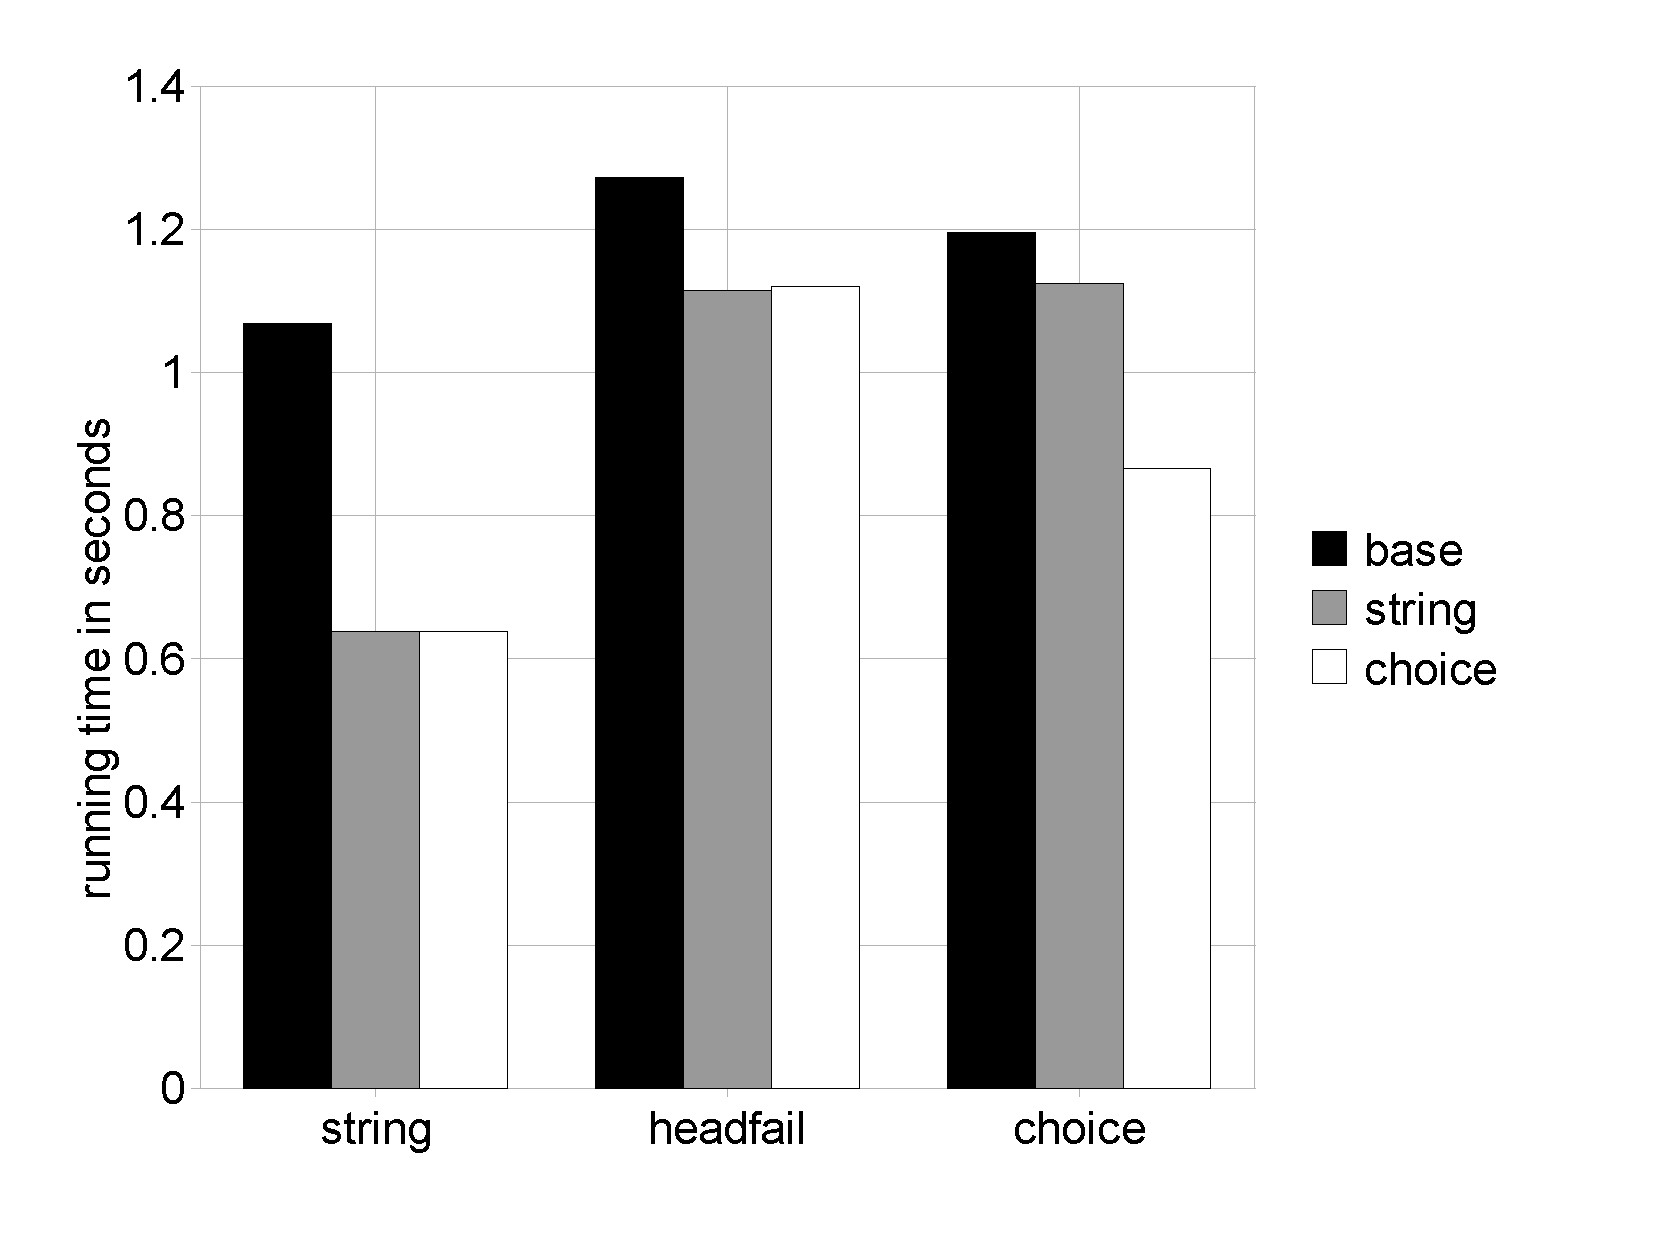
\includegraphics[width=0.49\textwidth]{microbench.pdf}
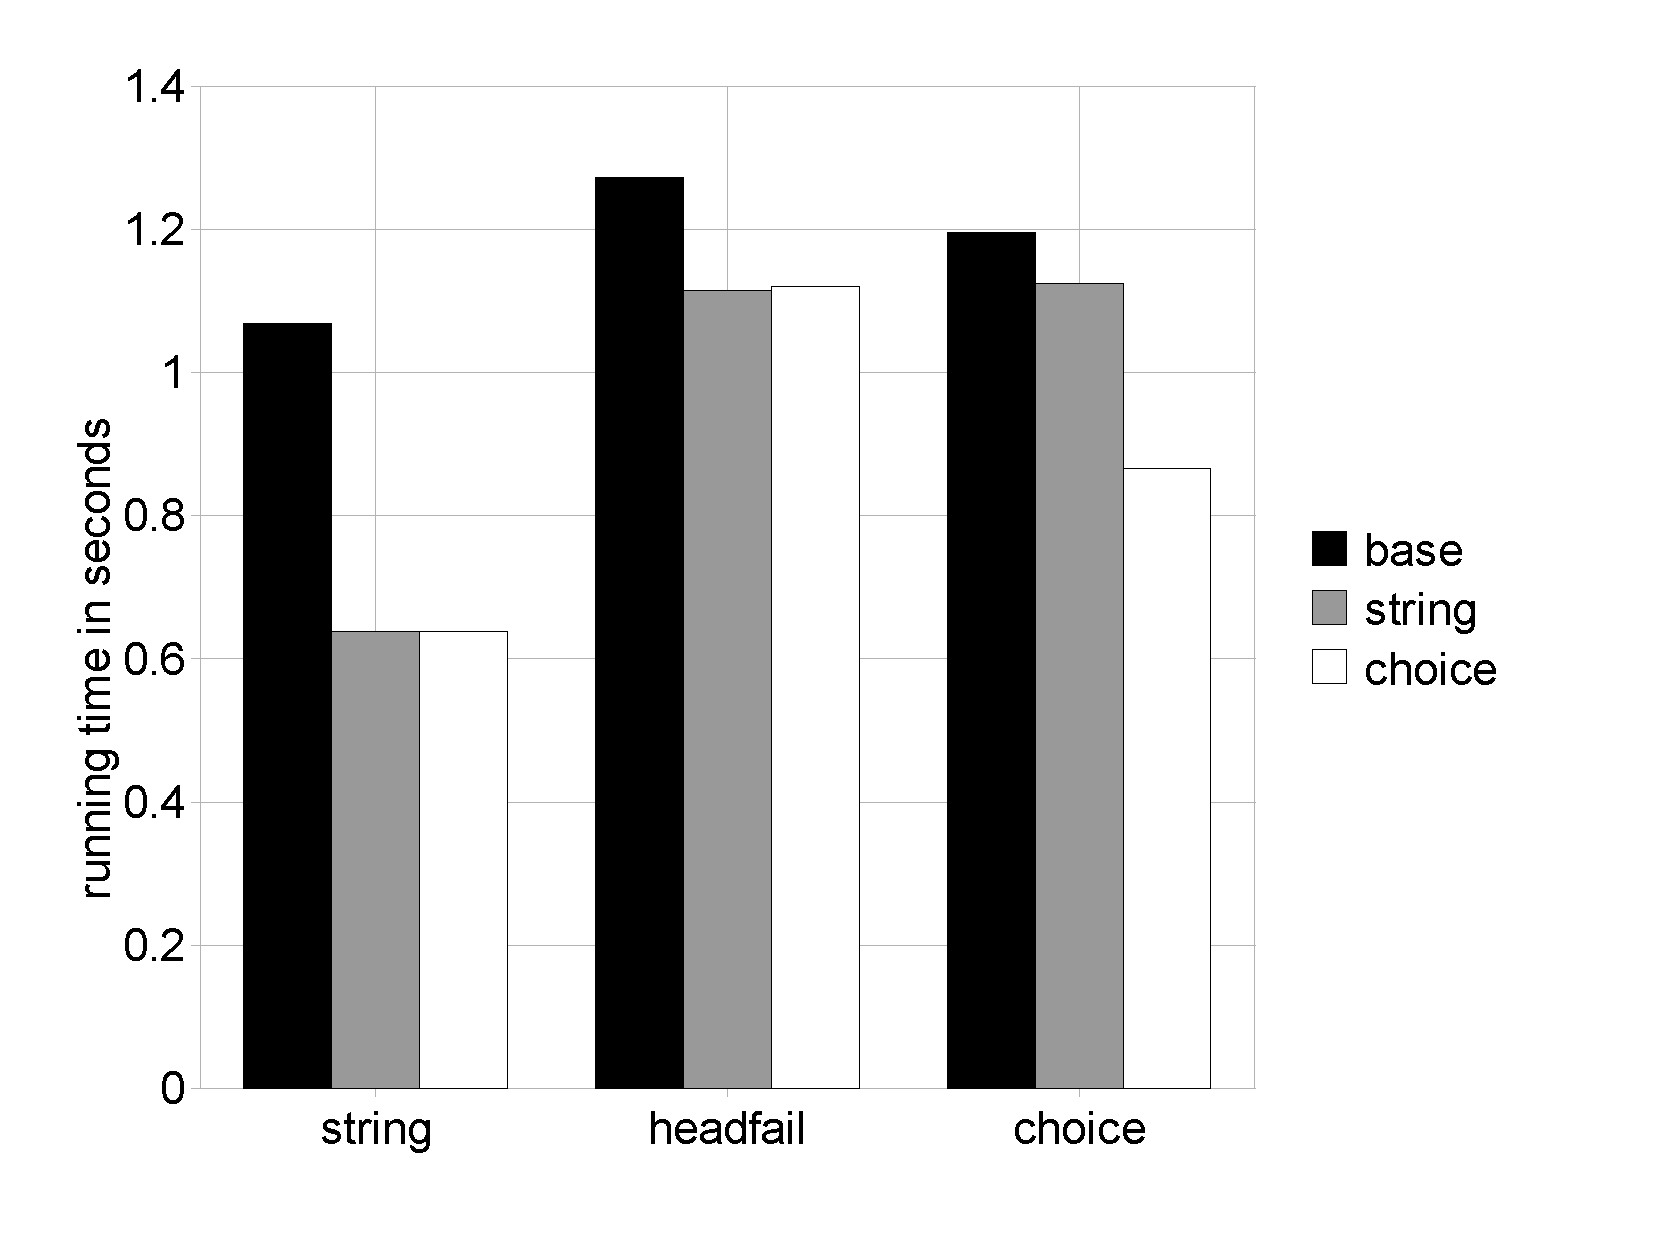
\includegraphics[width=0.49\textwidth]{microbench.pdf}
\end{center}
\caption{Benchmark results}
\end{figure}

\section{Related Work}
\label{sec:related}

OMeta is an object-oriented language that uses PEGs as a control 
mechanism~\cite{warth:ometa}, and is embedded in other languages (with
a JavaScript embedding being the most mature). OMeta also allows
pattern matching on list-structured data, and OMeta's authors have
an alternative operational semantics for list matching and semantic
actions for PEGs~\cite{warth:thesis}.

While in our semantics a match only produces values if there are
captures, in OMeta captures are implicit in the semantic rules (OMeta
patterns always produce values). OMeta also executes semantic actions
during pattern matching, so the programmer has to be careful with side
effects on semantic actions. 

OMeta has a kind of semantic action called a \emph{semantic predicate}, 
which can interfere with the match. We did not include it in this
paper due to space, but LPEG has a similar mechanism called a
\emph{match-time capture}.

Several programming languages, mostly in the ML family, include built-in pattern matching
facilities to help define functions over structured
data~\cite{spj:functional,spj:haskell}. The patterns are limited, not
providing any looping of repetition operators, or the ability to
reference other patterns. Pattern variables capture data from the
subject, and are bound to parameters of the functions.

Scheme has an implementation of pattern matching that works on lists
that is also primarily intended for destructuring
data~\cite{wright:pattern}. It has repetition, but
patterns still can't reference other patterns, so it also is strictly less
powerful than PEGs. Wright's patterns also can only capture data in
the form of pattern variables.

There are several languages for matching and validating XML-structured data that use
patterns to describe document schemas, one of them being \emph{regular
expression types}~\cite{hosoya:xml, hosoya:toplas}, an extension to
algebraic types that includes repetition. The patterns that describe
these types can reference other patterns (recursion is also
supported), but they are restricted to recognizing regular tree
languages, a restriction PEGs do not have.

Finally, parser combinators are a popular
approach for building recursive-descent parsers in 
functional programming languages~\cite{hutton:monadic1}.
Parser combinators combine simple parsers using operators such as deterministic
or non-deterministic choice, sequencing, chaining, etc. Although originally
designed for parsing character streams, parsing combinator libraries can
be trivially applied to parsing structured data. Their unrestricted
backtracking can have a large time and space cost (naive implementations are
particularly prone to space leaks~\cite{leijen:parsec}).

\section{Conclusions}
\label{sec:conclusions}

We presented an extension of Parsing Expression Grammars that allows
matching of list-structured data, instead of just character
strings, adding a \emph{list pattern} to standard PEG syntax. We
provided an operational semantics for PEGs with this new
pattern. 

Continuing a previous work, we also extended a parsing
virtual machine for PEGs with new instructions for compiling list
patterns, and proved the correctness of this machine and the compilation.
A few non-essential instructions were also added to the machine to enable two
list-specific optimizations.

We also added captures and semantic actions to PEGs, augmenting both
the previous operational semantics and the parsing machine. Captures
and semantic actions do not produce values, but promises of these
values. A separate evaluation step executes the captures and semantic
actions and produces the values. This makes side-effects in semantic
actions safe in the presence of backtracking.

We benchmark list matching and our optimizations on LPEG, an implementation
of our parsing machine for the Lua language. The optimizations are
show to be effective, and list matching using LPEG to be about as
efficient as a hand-written recursive parser, even when in the
presence of captures and semantic actions. Our benchmarks also show an
order-of-magnitude improvement over OMeta/JS, another PEG-based
pattern matcher that operates over lists.

LPEG has a richer set of capture patterns than we have presented here, such
as position captures (useful for error reporting), argument captures 
(useful for passing state to semantic actions), named
captures, and the math-time captures mentioned in the previous section. 
A formal treatment of these extra capture
patterns is straightforward and will be included in a future work.

\bibliographystyle{sbc}
\bibliography{sblp} 

\end{document}
